%%
%% Copyright 2007, 2008, 2009 Elsevier Ltd
%%
%% This file is part of the 'Elsarticle Bundle'.
%% ---------------------------------------------
%%
%% It may be distributed under the conditions of the LaTeX Project Public
%% License, either version 1.2 of this license or (at your option) any
%% later version.  The latest version of this license is in
%%    http://www.latex-project.org/lppl.txt
%% and version 1.2 or later is part of all distributions of LaTeX
%% version 1999/12/01 or later.
%%
%% The list of all files belonging to the 'Elsarticle Bundle' is
%% given in the file `manifest.txt'.
%%
%% Template article for Elsevier's document class `elsarticle'
%% with harvard style bibliographic references
%% SP 2008/03/01
\documentclass[final,5p,times,twocolumn,authoryear]{elsarticle}

\usepackage{graphicx}
\usepackage{amssymb}
\usepackage{listings}
\usepackage{nameref}
\usepackage{minted}
\usepackage{csquotes}
\usepackage{rotating}
\usepackage{hyperref}

% DEVELOP ONLY COMMENT BEFORE SUBMIT
\journal{Astronomy and Computing}

\begin{document}

\begin{frontmatter}

\title{ AstroOD: A Peer-to-Peer Electronic Cash System base-layer for the Open Development of Astronomy: Education and Research}
%\subtitle{Towards the open development of astronomy through a Blockchain based smart token}
 
    \author[iate,wsu]{S.Gurovich}\corref{mycorrespondingauthor}
        \cortext[mycorrespondingauthor]{Corresponding author}
        \ead{sgurovich@unc.edu.ar}
  
\address[iate]{
   Instituto De Astronom\'ia Te\'orica y Experimental -
   Observatorio Astron\'omico C\'ordoba (IATE--OAC--UNC--CONICET),
   Laprida 854, X5000BGR, C\'ordoba, Argentina}
\address[wsu]{
   Western Sydney University, Kingswood campus, NSW, Argentina
}

\begin{abstract}

An interoperability catalyst or (Open) Development driver based on (Open) Blockchain technology is considered for Astronomy \& Astrophysics Education, Research and Development from K-12 through to the tertiary research level. The challenge for the community is to build a store-of-value and value-added programmable incentive layer upon open Blockchain protocol standards. Although the main motivation as argued is the steep decline in the half-life index of PhD Astronomy majors' in the  public University system, (United States - taken as  proxy), open development tokenomics and governance protocols should enhance growth in value, auto-regulate, minimize and mitigate other negative features that affect and hinder open development in Astronomy that might be rooted in centralized decision making. It is proposed that this alternative Open Development Stack be based on the Nakamoto Bitcoin standard and other Open block-chain based networks, including the Decentralized Finance Movement, identified to be disrupting Central Bank/government issuance of FIAT currency as an alternate 'sound money' proposition, and if FIAT issuance is as it appears to be by some metrics is proving to be a factor or barrier to Open Development (OD) then an alternative and complimentary funding mechanism based on DEFI liquidity should naturally help drive OD in Astronomy, our assumption. An counter proposition is that DEFI is a front-running industry that does not have much future for Open Development from which it was born and is not part of the open protocol stack.

Another key open-ended question results: 

If Open Blockchain technology is a way forward to store, protect and enhance value in Astronomy then what protocol properties and governance strategies might be effective?

Some case-study 'events' are identified. Metrics that track Open Development are proposed that could be refined over time by the community. Some risk factors at World; National; Provincial/State; University level;  etc., of governance are examined and case-studies presented some of which have led to astronomical communities failing to enter or even maintain international collaborations on global projects or facilities; or led to a so-called 'global' brain drain or flight of Astronomy majors to other industries, caused interruption of unique telescope facilities from normal operations or delayed construction of new ones. 

Our model, serves the following actors that are part of an already burgeoning "Open Source" Community: Astropy, National Public Universities and other astronomical institutions as recognized by data-feeds from existing protocols: eg; google-scholar; NASA-ADS;  whose weighting as proposed should be configurable, and managed via WEB3 enabled DAPPs, by the community. Other international founding parties identified include; The  International Virtual Observatory Alliance and the International Astronomical Union. A function in smart-contracts could be used to delegate votes from individuals, in governance polls, an example of such code in a ERC20 contract is given.

For AstroOP, DEFI liquidity should be sought periodically from Decentralized Exchange(s) eg: Curve Finance, UNISWAP, and other DAO as considered by the community: The case however is that AstroOD be seed funded by DEFI, including UNISWAP Treasury and Education funds, \href{gitcoin grants} {https://gitcoin.co/grants/}, etc.,.  Some final use-case are presented including a case-study to include an NFT series to celebrate aniversary milestones in historic astronomical institutions. An example is given as an NFT series for the 150 year anniversary of the former Argentine National Astronomical Observatory or to mark the historical event of the 1912 Solar Eclipse expedition that set out to constrain Einstein's GTR, led by the then director of the Argentine National Observatory - Perrine 1912, with a message signed by Honorary IAU member and historian Santiago Paolantonio and another case-study of a conference NFT to fund prizes, travel grant unlocks., etc at the Institute of Theoretical and Experimental Astronomy's (IATE) Friends-of-Friends Annual Meeting. 

% technology is a natural evolution of The Computer as proposed by Vitalic Buterein then it stands to reason given the tight connection between astronomy and technology that at least in the academic ecosystem such discussion should at least be had. 

%To the end of a Token for Astronomy, basic discussion of a road-map is had in this paper some identifiable issues as protocols for Astronomy "open-development" discussed. 

%Based on some generic smart-contracts. Initially this tech is proposed to have a direct influence on financing and execution of STEM careers  and to revert negative features of the current model that like the Half-life decay of Astronomy PhD majors as determined from statistical studies of US Public Universities. Since the US Public System is large and other similar systems based on it. The current Astronomical Development Model identified to be based on more Centralized Governance that relies on National Fiat Budget approvals, so a feature of our model is that a value-system based on Bitcoin and Ethereum who have each had ROI over the last decade superior to gold or most if not all other asset classes, that the old Meritocratic development Heuristic model often with "Elephant in the room" system failing such as in funding crisis, governement budget warfare, lawfare, debt and crisis that affect directly STEM research and such scientific development is defined to be 'closed' as opposed to 'open'. The old 'closed' heuristic often is often affected by cyclic economic crisis, currency devaluation, unemployment with real affects to the population, such a Heuristic of development challenged in this paper are based on political partism, centralized systems of power giving rise to the Military Industrial Complex, Petro-Dolar inspired drug wars (Chomsky, Understanding Power). Open Blockchain, anti-censoring technology is proposed and in particular through the perspective of thought of a new straw-mans-model as a natural evolution of Astronomy, piggybacked on Open Development Scientific Stack including the fast developing Decentralized Finance Movement, as at worst another useful system to incentivize real value development in Science by programming it to be more open.  

\end{abstract}



% Techniques based on artificial intelligence or machine learning has meant that precise data feeds or meta data eg: IRAF II standard, has shown the importance of synergy between new (Centralized) and optionally (decentralized) Scientific Research endeavour. 
%The current limitation of funding and crisis in Scientific development faced by the foot-soldiers or perhaps someone colloquially described "data slaves" motor of scientific technical development mostly brought to bear by Science Major Career graduates. Since Open Development rests on the Tenets of open source, and given a significant percentage of astronomers use Astropy for some data analysis so we propose an affiliated package of Astropy hereby called astroOD, to be used to create and manage individual wallets and transactions of Fungeble and Non-funagable tokens that serve the Open Developemnt of astronomy.  Although initially astropy users and developers will be onboarded, we propose a staged onboarding setup for successful implementation across the wider astronomical community. Many parts of the tokenomics model are taken directly from the so-called 'decentralized finance' movement that allows for the development of decentralized applications (DApps) on mobile devices to facilitate transactions, transparency and usage of the blockchain via astroOD Tx. This paper investigates possible protocol standards and discusses cross chain technologies via Oracles as a technology applicable to validate transactions and safeguard value via data feeds (Eg ADS searches, citations, etc.) and explores the concept of guardian nodes. General background conditions that motivate adoption by the astronomical community of such a system are presented as some model component parameters. Other technical details are omitted and not fixed but could be be soft or hard-wired after successful vetting from the governance component by means of periodic voting based on staked amounts A staking system is discussed to finance successful projects and  potential governance actors with initial staking claims including members seemingly outside of the astropy development community: Universities, National observatory facilities and institution, amateur astronomical associations, International Astronomy bodies (eg: IVOA, IAU), primary and secondary schooling bodies and other official and unofficial actors that promote astronomy research, education and outreach are discussed.. 



\begin{keyword}
   Astroinformatics \sep 
Blockchain \sep Open Development
\end{keyword}
\end{frontmatter}

This paper proposes adoption of public blockchain ledger technology as a value optimization (and complimentary) base-layer for the Open development of Astronomy. A comprehensive review paper of blockchain technology with primitives can be found in \cite{20d30b4efb014b21b7ab27f5218692ab} and references therein. In our Straw Man Proposal Study, although the purpose is for the open Astronomy development, other STEM communities may also consider it of interest since Open Source protocols are burgeoning and synergies and parallels already exist [See HapMap project and its Open Source dependence for the human Genome Project, \cite{GITTER2008529} to prevent closed patenting licensing]

%In the last dozen years any community that built its value system on top of the Open Public Ledger stack that itself is based on The Bitcoin Standard Protocol would be wiser for it. In this paper, an attempt is made to bring to light into the debate interesting Blockchain primitives that have been largely unexplored but based on Open Source Development, to fork to existing protocols to promote interoperability through data-feeds, no doubt equivalent to  "ADS, Journal pub", IVOA protocols, etc identified in our case for Astronomy, to be seeded through "open-development", by the Community for the Community and through Layer 2 decentralized governance solutions.

%Potentially Blockchain technology for open development will continues to be more important so it could be argued that "Computer Systems" hardware and software will continue t evolve because of Blockchain, as shown in ASIC hardware development, increase in Pico Hashes per second surpassing Moore's Law and by the fact that Blockchain technology is is heralded by its proponent as disrupting the global financial system as evidenced since the first Bitcoin Block and through the last decade. 


%One of the problems of `Astropysics' which was an astronomy python package maintained by Eric Tollerud who is one of the OG of Astrpy, was that although projects were open there where many developers that maintained their own packages and had functions that often were similar or if not the same. This meant that less than efficient development of code could take place. 

%In an TCG IVOA meeting. Erik presented some evidence that IVOA development is sometimes a bit skewed to the big projects like ESA, astrogrid (UK), perhaps two of the most influential International Members of IVOA. These projects even design space-born telescope/instruments with multi-billion dollar buldgets. Unfortunately at times some of the standards that emerge are not exactly optimal for the communtiy most of which (70 percent, Tollerud) as shown in a recent poll work as data analysis using Python and the astronomical libraries of Astropy.

%Any complementary base layer model must be able to react to systemic risk factors to open development and sufficiently robust to build-up immunity to mitigate against counter-party risks that could be rooted in Financial; Health (Pandemics) ; or other political motivations that hinder Open Development in Astronomy. Some case-studies are discussed. 


    

% =============================================================================
% SECTION INTRO
% =============================================================================
\section{Introduction}
\label{sec:intro}
%
 It is now generally agreed amongst Computer \& Data Scientists that perhaps the `first' identified computer contained the Antikythera mechanism, that was re-discovered in 1901 from the debris of a ship-wreck that has been estimated to have occurred about two thousand years ago. \citet{Freeth2021} and other studies therein have demonstrated that the Antikythera mechanism was designed to solve mostly astronomical problems based on a technology that rested on much theoretical support from Ancient Greek Astronomers. 
 
 The Antikythera `computer' contained three finely crafted rotating discs and thirty-odd cogs that were all designed with adequate tolerances to calculate and predict the relative positions of some Astronomical sources including The Sun and The Moon, from different locations of The Earth. These constraints were set mostly for navigation, agriculture and spiritual reckonings. 
 
 Today, Alan Turin (AT) is recognized as a modern father both of `The Computer' and of `Data Science' for his pioneering work in the twentieth century; that paved the foundations of Artificial Intelligence (AI) and Cryptography. To astronomers, `Machine-learning' and `Data Mining' AI techniques have proved beyond any doubt effective in revealing physical insights or the physical parameter space of astronomical sources in The Universe from ensembles of data measurements in the observable parameter space. AI techniques have been used as effective tools in thousands of published studies found in the literature. What is perhaps less well known, is that due to the incoming data Tsunami produced by new surveys and data pre-possessing requirements for real-time data clensing, AI techniques are possibly now playing a critical role in the evolution of Astronomy: eg Vera Rubin Survey Telescope, and Square Kilometer Array pre-processing data pipeline. On the other hand cryptography other than as a tool used for compression and data access security; has not been much explore for Astronomy development. On the other hand, in this paper cryptography and blockchain is proposed as an essential complementary base-layer for the open development stack of astronomy. 

Our goal is to discuss use of Blockchain technology in a `Straw Man Proposal' as a primitive base-layer stack for the Open Development of Astronomy.

 \begin{figure}[h!]
    \centering
    \label{fig:cowenbtc}
  \caption{Historic Price function (in USD) of BTC in time (Years), as a potential underlying store of value for Astronomy development. The color-bar is a risk metric modelled by Cowen et. al; (2021)} for 3 previous different market-cycles that relate to the bitcoin halving mining reward.
  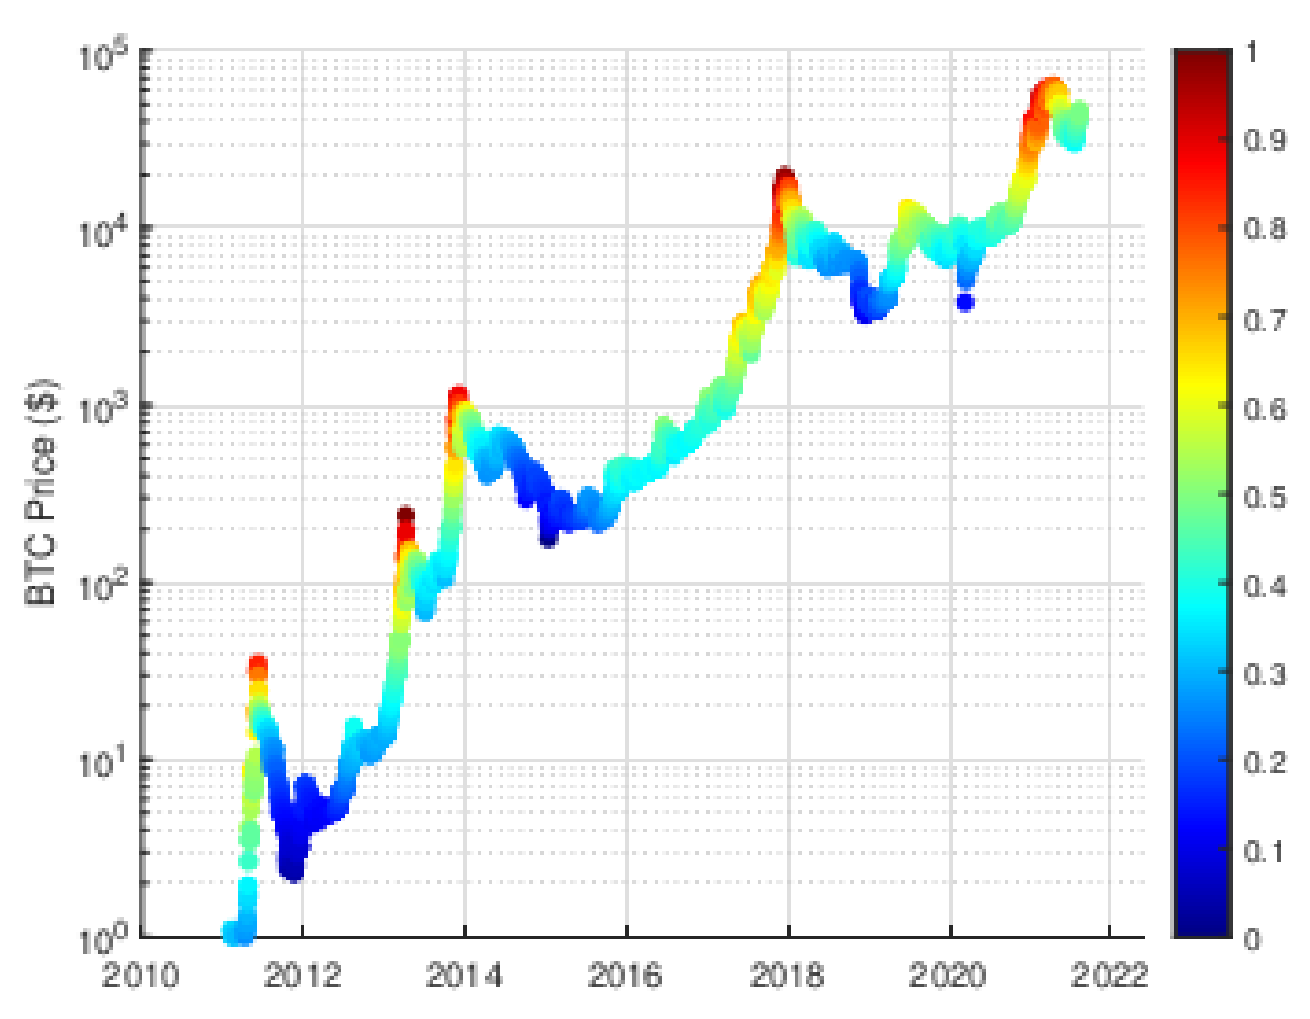
\includegraphics[width=0.5\textwidth]{figs/cowenbtc.eps}
\end{figure}

\begin{figure}[h!]
    \centering
    \label{fig:crisis}
  \caption{Historic global Crisis, Figure taken from \href{https://en.wikipedia.org/wiki/Global_recession}{wikipedia-commons} adapted from data Reinhart and Rogoff (2009) depicts the binned instances of global crisis (Y-axis) for individual countries that grew in number exponentially before and after the US Nixon administration pulled out of the Breton Woods accord unilaterally that required physical gold backing to USD money printing.}
  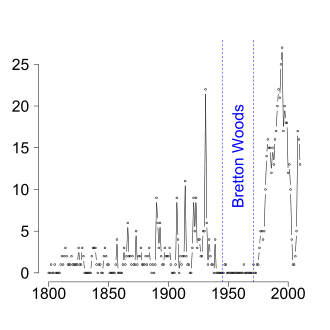
\includegraphics[width=0.5\textwidth]{figs/330px-BankingCrises.svg.png}
\end{figure}

\begin{figure}[h!]
    \centering
    \label{fig:F4.large}
  \caption{Figure taken from Milojević et al.) depicts the falling half-life rate in Astronomy and Astrophysics and other STEM fields}
  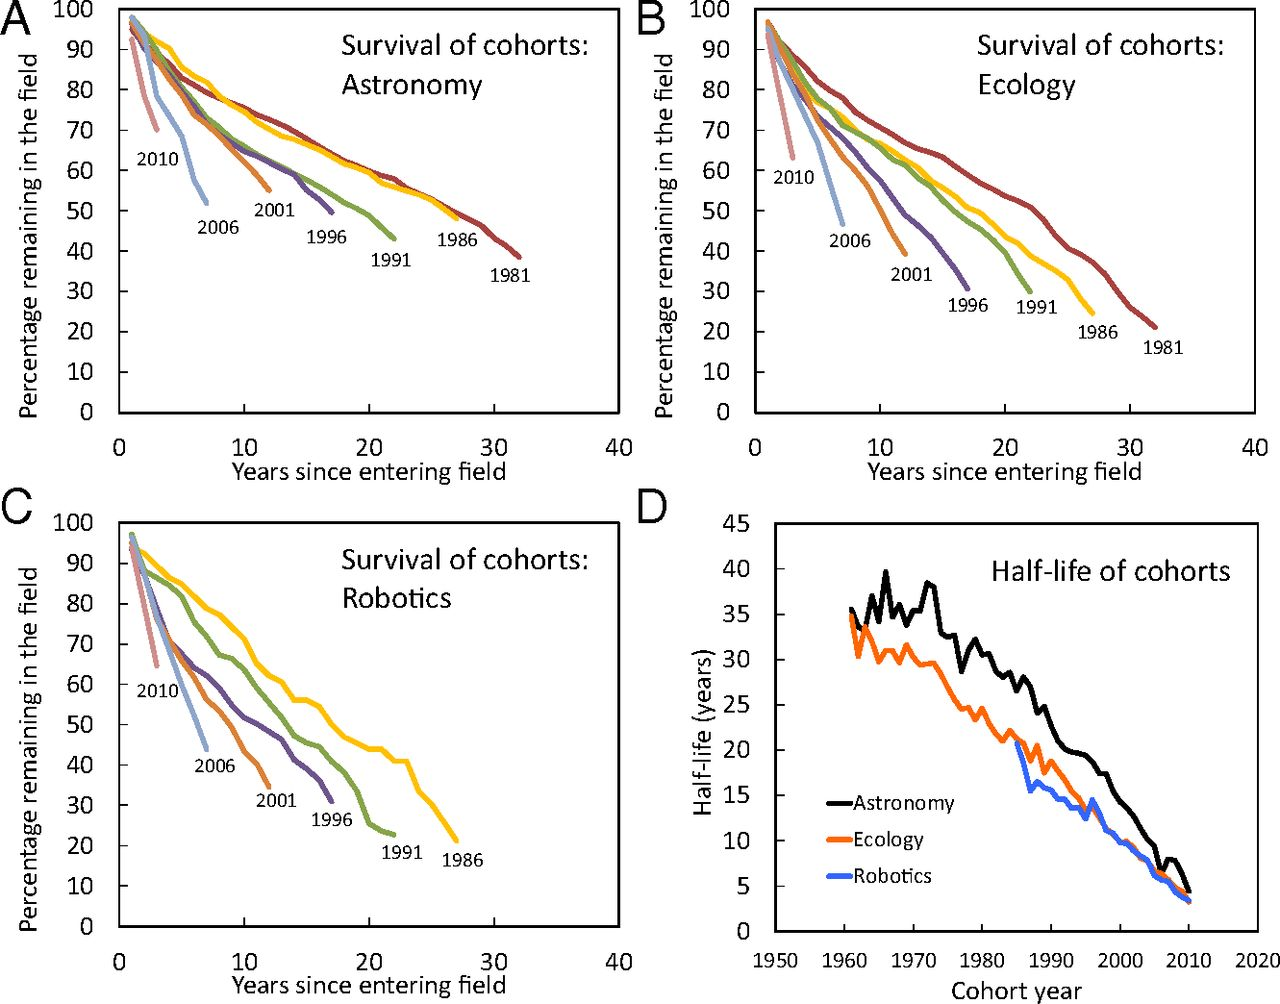
\includegraphics[width=0.5\textwidth]{figs/F4.large.jpg}
\end{figure}

\section{Blockchain Review}
\label{sec:bc_review}
\cite{20d30b4efb014b21b7ab27f5218692ab} present evidence as do other authors therein that Blockchain technology is much rooted in academic studies. Their fig 1 show a time-line preceeding DEFI in which advances in blockchain primitives can be found here \href{https://queue.acm.org/detail.cfm?id=3136559}{ACM}. 

This model is inextricably tied to the BITCOIN standard. A review can be found in \citet{Hansen2020Book}. Aside from the Nakamoto block size constraints to allow full-nodes to be run on a single PC, several other properties entitle its selection: Since inception in 2009 and after 12 years of price action (see Fig 1) it has proved to be a valid store-of-value far superior to the USD standard that has had a high cost. Although in the short term, (months or less) there is volatility and the BTC/USD pairing is somewhat correlated to global financial markets, in the long term volatility is falling and so for solution to the case-studies included this paper,  BTC is a reasonable choice for the base layer store-of-value. In the range of a decade it has been the top performing asset, even superior to gold. It can be operated on globally, 24h a day, 7 days a week. Given the Tx requirements for many applications for the open-devlopment of astronomy where Tx costs are an issue other Open blockchains can also be used for technological-operational issues, since the small block-size of Bitcoin is as designed less flexible, scalable, etc allow a full node to be run on a PC. Market cap, ease of use, developer numbers, technology standards, cross chain Tx, as well as other indicators of other chains must be considered including Ethereum, DOT, LTC and other blockchains. Some of these other chains have thriving developer communities, DApps and have billions of USD in locked liquidity from the very Decentralized Finance Movement, a purposeful central tenet of our model. Ethereum's smart contract programs and Oracle solutions are also considered as base layer technology for our governance protocols. Having prediction market protocols to help develop Astronomy must be contemplated and developed by The Community to mitigate stochastic ill-effects to development.  We show in Fig 2 the Global crisis function that depicts an exponential increase in crisis when no suitable global reserve is issued, that was not the case during the Bretton Woods accorded period. We propose a complementary underlying value system and claim to tie it to the BTC as our model's go-to store of value of Nakamoto et. al. and BIPs. In Fig 3 we republish the half-life empirical function metric for astronomy and astrophysics PhD majors at US Public Universities that shows the alarming exponential decline.  In Section \ref{sec:btc2}, discussion of the current and historical situation that has underpinned the negative effects of Astronomy development with examples is discussed. In Section  \ref{sec:btc3}, some blockchain primitives and protocols are identified, selected to complement Open Astronomy Development.  In Section \ref{sec:btc4} a simple idea of implementation and on-boarding for our model of Astronomy education/development and research via open development is proposed via Astropy, the leading Open Developer community tool-kit by Astronomers for astronomers. In Sec. \ref{sec:btc5} conclusions drawn and some discussion on a possible future course of action, plus an NFT case-study to celebrate 150 years of the Observat\'orio Astron\'omico de Cordoba, the former National Argentine Observatory. 

\section{Open Astronomy development}
\label{sec:btc2}
The half-life of about $\sim 3$ years for Astronomy majors in US public universities is an alarming metric. It has been dropping exponentially since about 1970 or about the same time the US withdrew unilaterally from the Bretton-Woods accord that tied the 'price of one USD' to an allocation of gold. This desertion rate metric could be considered a global hemorrhage of 'grey matter' capital or the so-called hidden 'Brain Drain' to astronomy development. 

We contend that scientific contributions from the community should be protected, valued and enhanced in a P2P application-layer sense by choosing a more robust gold2.0-standard programmed by the community through open governance.


We recognize that Blockchain technology rests on the Open Source stack because it includes a tried base-layer community developed protocol and recognize Nakamoto 2009's white paper on this subject. In the last decade Open-Source projects in Astronomy have burgeoned and become somewhat unified. 'Astropy' and its community affiliated packages has become the leading community colaboratory dev repository tool.  One of the reasons the community got behind one project was that many packages offered similar functions and the maintenance costs scaled with the number of version. Some methods may have been more optimal, so a standard system evolved, that now maintains the code base in the community. In Astropysics the main developers realized with other members of the community that community maintained code repositories was key to Open-Source Development.

It is contended here, perhaps somewhat heuristically that like The Computer that has continued to be a fundamental tool for astronomical problem solving, although most astronomers use Astropy amongst other tools, no block chain modules yet exist on Astropy so we content one must exist and propose AstroOD. 

Could a value added Astronomy Token that rests on the evidence of over 1 dex and achievements in Decentralized Finance (DEFI), because they are based on BITCOIN and ETHEREUM asset classes that have outperformed gold in this time prove useful in this task? Ie lend to funding and technology of DEFI instead of from Bank loans underwritten by governments?

 
Could a "World Computer", reference Vitalic Buterin, help solve the crisis in PhD degree careers as seen exacerbated in as many a dex (see Fig 2), in some natural and applied STEM fields as ,demonstrated by the exponentially increasing desertion rate?

Figure 1 shows the financial crisis recorded about the Bretton Woods accords, when US unilaterally pulls out.

Before Bitcoin some initial attempts of a digital currency yielded successful prosecutions by the US Fed court system vaguely under the term: 'Counterfit' of the legal tender or of the Fiat currency system. 

Source:  
 
\section{Early protocols}
\label{sec:btc3}

Early store-of-value protocols preceding BITCOIN are discussed in Chaum (1983), Chaum, Fiat Naor (1989), Rivest and Shamir (1997). Haber and Stornetta (1991) discuss the notion as an important driver for global scientific, social and cultural growth that with 5G promises to rival the historic highs of 18 \% of World annual GDP of the likes not seen since the first industrial revolution (Walden et al. CTO of NOKIA, Bell's 2018 speech).

If Bitcoin/Blockchain is a decentralized technology, its use as a store-of-value for Astronomy must complement decentralized education research, and development. This is embodied in the so-called term: "Open Development".

 
However, in the first decade of the 21st century came Bitcoin, published anonymously by Satashi Nakamoto in 2008.  In the first block, see Figure 1: is a reference to the New York Times article that claimed The Chancelor considering a second round of Bail-Outs for the biggest British Banks. Satoshi, it could now be argued is a pseudonym. According to some analysis probably represents the work from mostly one person (MOOC BlockChain, Princeton). Never-the-less Bitcoin and it's Blockchain appears to have generated a store of value over other asset classes so it could be seen as a Market fact thus far in time-frames of years in it's first decade of existence the Store-of-value proposition appears to be holding. Recognizably in shorter time-frames (days or even months) BTC volitility is higher. Some authors argue that as an asset class since it is measurably young it is also tends to be more speculative that should become less volatile in about as long a time-scale (years, decade), asset (Antonopoloulos)? Energy Usage is also discussed here in Section XX. 
 
BTC as a world reserve still appears to be partly correlated to other global financial markets. A recent example is the Covid19 black Thursday pandemic effect that in March 2020 saw BTC price drop by more than 30\% in only a few hours. This appeared to be triggered by the Black Thursday liquidity crisis that swept the much larger global financial markets and the reactions of central bank governments to it. This time coincided some of the more valued equity market stocks suffered the worse losses since The Great Depression" and iconic corporations were "bailed out", like Hertz after a record number of unemployed, filed for unemployment benefits in the US. After about a fortnight, like many blue-chip stocks, bailed out by the US FED via Repo, corporate bond offers, and share buy-backs the BTC US stock price indices recovered almost instantly. Against other asset classes including gold and USD, BTC appears to be in the short scales at worst, as volatile. 
 
 
Bitcoin as a technology to solve several problems faced by earlier digital currencies. Having no single point of failure meant law suits can not be used to persecute anonymous creators. This adds to network security by processing Hash functions which is adjusted on a two week basis. Some authors, including Andreas Antonopoulos believe Bitcoin and Ethereum blockchains have the potential to revolutionize open development in science and technology and with 5G roll-out promise unprecedented levels of growth of over 18 percent per year, not seen since the first industrial revolution Waldon, M.  Fig needtoinsertfigure adapted from Walden et al. shows the world GDP as a function of time. These technologies were born out of academia, the occupy wall-street and anonymous movements as a direct response to the 2008 financial crisis that saw a global slump in the world GDP based on the US sub-prime financial crisis  that included a drop in US GDP by 30 \% sustained over several years.
 
Programmable money is not exclusively relevent to human beings but also to machines as particapative actors. Hardware evolution is also tied to open development, as seen in the evolution of specialized hardware architecture for Proof Of Work (POW) HASH Function calculations that is developing Application-Specific Integrated Circuit (ASICS) to mine Bitcoin blocks. It could be argued that these developements have outpaced Moore's law.  Wrights Law suggests that the for every percentage increase in the cumulative distribution function of production in any industry equates to a fixed percentage increase in the efficiency of production. So hardware has evolved from CPU intense through to graphic processing units (GPU) and  Application Specific Integrated Circuit  (ASICS), \cite{10.1371/journal.pone.0052669}. A successful model for Astronomy and Astrophysics Open Development would do good to tie metrics of Open Production into the protocol as well as the appropriate incentive mechanism.       

Open Blockchains are uncensored so a data protocol standard of best practice through governance could be cross validated from an information criterion perspective that includes Oracle feeds for Open Development.  Oracles that receive feeds are penalized if they predict incorrect probability distributions of events or Facts for Astronomy Development prediction markets. 

\section{Early Blockchains}
Turing complete programming languages like ETH (ref to Vitallic) but unlike BITCOIN  (refernce to Satoshi) have loops and are able to iterate infinitely.  Bitcoin was purposely built to be much simpler, it has proven in just over a decade (see Fig \ref{fig:btc}) to be a good store of value when compared to the USD. It does not deal naively with Smart Contracts. Although Ethereum can do much of what Bitcoin can, its scope is far larger than simply being a digital, decentralized global store of value mechanism of human transactions. Whereas Bitcoin was primarily designed to be a P2P form of electronic cash, the Ethereum blockchain was designed to also function as a “World Computer”. There are many excellent sources in the Literature on this but we will concentrate on Atributes of a Token for Astronomy in the Section below and describe aspects of our model.
 
% \begin{figure}[h!]
% \centering
% 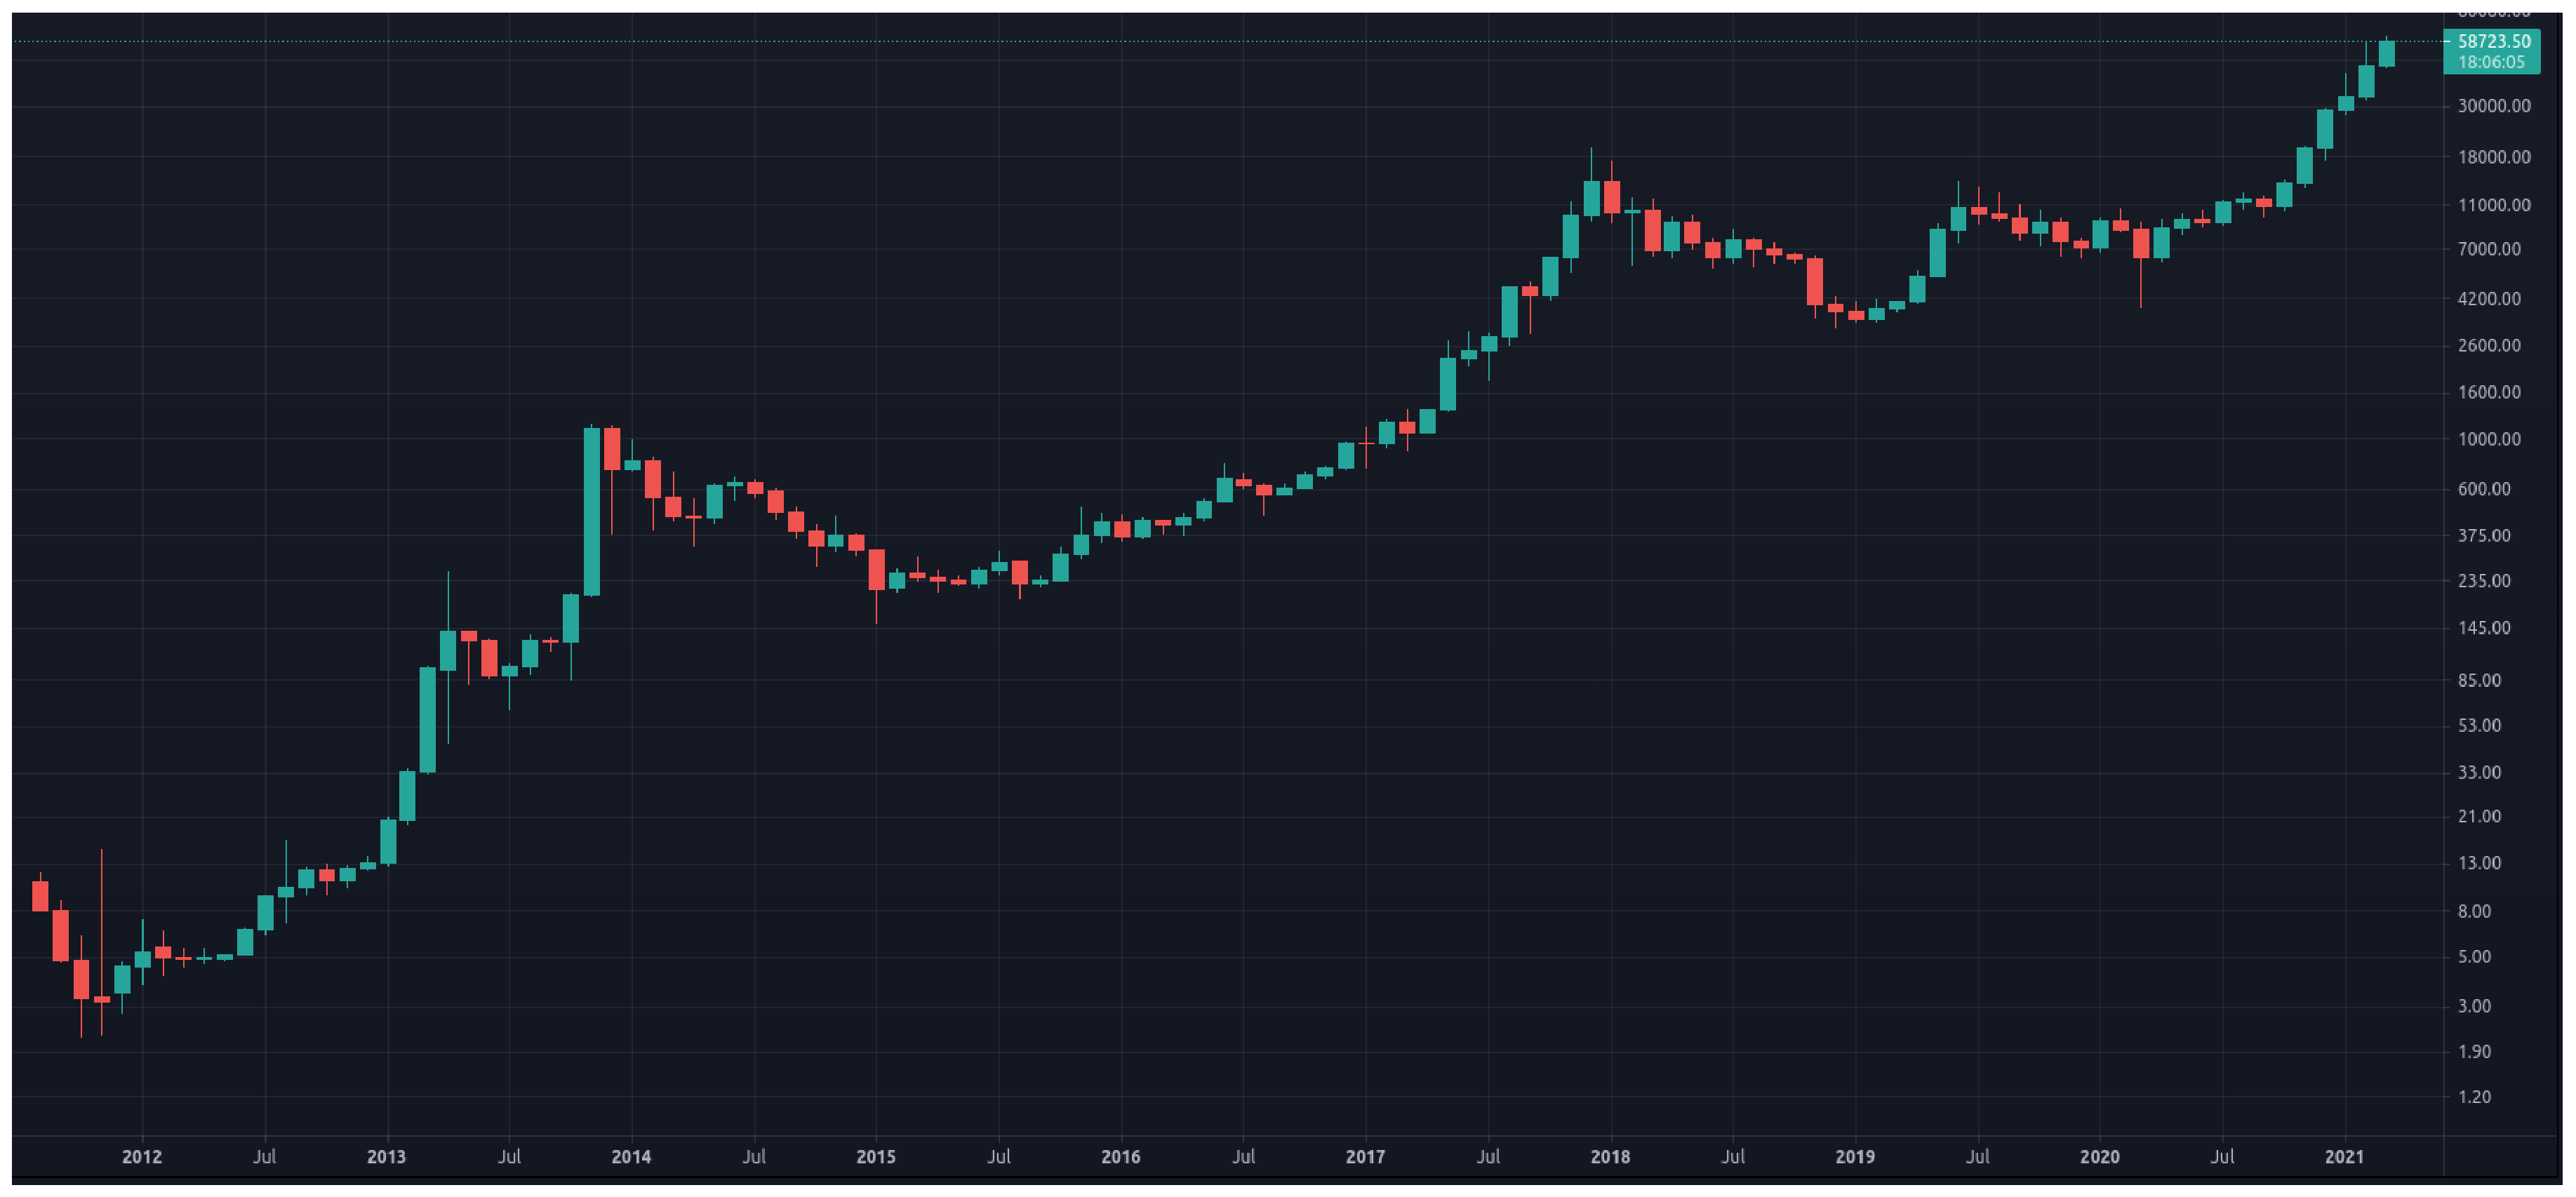
\includegraphics[width=\textwidth]{figs/btusd.eps}
% \caption{BTC/USD}
% \label{fig:btcusd}
%\end{figure}

\section{Indexing Production and Development}

Community validated production metrics would form an important basis for any Open Development Model in Astronomy that is the focus of this paper. These metrics can be used to supply liquidity for the Open Development of Astronomy.  

We choose protocols from the Stack of DEFI protocols as a Starting point since if DEFI is really the basis of decentralized Open Development then by using these protocols when there is a need identified by the community as a dynamic should naturally flow, a type of Lindy effect justification of using proven, tried and resistant base-layer open development protocols, methods and procedures.
 
 \section{Model Attributes of a Token for Astronomy}
\label{sec:btc4}
RSA Ecliptic Curve Algorithm, asymetric hash function, Blind, Schnor Signatures, Merkle Trees, ZKP,  WEB3, Multi-sig, Cross chain, mixing - Privacy. 

\subsection{Block Validation}
\label{subsec: validator}
Blockchain Validators and Nodes. ERC20 Protocalls like GRT ERC   

\href{https://defipulse.com/}{DEFI$\;$ PULSE} pulse is a list of all the liquidity that is tied into DEFI. There is over 77.77 $\times 10^{9}$ USD locked in DEFI. In the UNISWAP treasury there is about 3 billion dollars. These treasury funds are available via grants programs that Astronomy Open Development protocols should have access to.

In this Section, a toy model for the open development of Astronomy based on open Blockchain technology is presented. An attempt is made to sketch out ingredients and methods of a `successful' model. Some elemental principals as voted by governance should be voted at different stages calibration proposals. For argument sakes in this model we follow the UNISWAP snapshot community, where there are different instances of governance. We also have a treasury funds, and the like.  through governance solutions. The UNISWAP model, to date is one of the largest decentralized exchange, has many developers working for it, was the first massive airdrop token of blockchain value, so is essentially decentralized in our assumption. The funds for this Paper come from DEFI, from the NOVA node of the IVOA-EXEC committee for Argentina. Some fundamental actors are identified and their functionality with the model sketched out. This paper does not pretend to discuss in strict technical details the finer points of the implementation of such model and parameters therein, but does make reference to some basic cryptographic primatives including Merkle Trees, Zero-knowledge proofs, cross chain protocals, etc. that offer promising solutions and could certainly be considered to be incorporated during Improvement Proposals directed by the community periodically. The paper does not delve into technical details of some blockchain procedures like mixing to maintain secure personal and private information but of all actors but pretends to highlight some core model features to be followed up by future authors but obviously  locked value will naturally flow to the more useful protocols.  
 
The only condition to participate is bonafide scientific curiosity for Astronomy so sufficient incentive methods need to be developed to entice value-added interaction with the astronomy blockchain via Decentralized Block Chain Applications, (DAps) as programmable parameters that can be set by the Model's governance component albeit individual minority actors. 

For the sake of simplicity the following three `actors' are identified as founding governance members: International Virtual Observatory Alliance, the  Astropy community and authors of referred peer reviewed journals weighted by their h-index, the International Astronomy Union etc. Parameters such as the weight of each should be set soon and be discussed by the community. The reward will be the AstroOD Token, since the wallet creation, blockchain exploder and DApp python tools and protocols are unified by the proposed affiliated package of astropy. This parameter could be considered to as a proportionality of any initial coin distribution function. But we would be against this and think programs need to start from the ground-roots up, providing liquidity and rewarding Tx were useful (community validaded) Tx occur. 

Over 70 percent of Astronomers use  Astropy and since it is recognized as a go-to for Astronomy Software Development so the Astropy Community is chosen as founding actors of the Open Development model (here-after ODM) of Astronomy as proposed. Affiliated package authors could be validated and offered a period to open a wallet and partake in governence DAO. An affiliated package to Astropy is selected to generate private public SHA256 pairs and the generated funds will be locked by the Community 70 percent to Developers. 

The AstroOD package 

We propose an AstroOD affiliated package \textcolor{red} github ref. that when Log switch is turned on collects basic statistics of packages being used and is correlated to ADS Main-Text query and ORCID query. Anyone in the Astropy community can create key pairs to be used as Smart Contract accounts. The program using RSA, and blind signature for privacy. The package will include a functional wallet, with multi signature, multi currency and multiple accounts. This will be the basis of deployment of “Smart Contracts”, as a concept was introduced in 1995 by Nick Szabo, who described Smart Contracts as “a set of promises,
specified in digital form, including protocols within which these parties perform.

AstroOD package will have to be built to implement the use of Oracles, to connect the community to the blockchain space. Oracles manage feeds of information are not put into the native blockchain due to scalability or privacy issues, etc but to other Chains.  Oracles are more focused on price-feed data for crypto asset prediction markets but with DEFI burgeoning and necessity the Oracle inputs are becoming more diversified.  The Oracle Problem 4 promises” (Szabo, 1996). 

Feeds for Oracles would include ADS-NASA, ArchieX ., etc,  to validate information that can be used to automatically set parameters in the model. The weights could be voted on by IVOA representatives.

If the  model truly represents an open blockchain then anyone can participate and be offered rewards as incentive in pursuit of open astronomy. It is obviously important that protocol standards be defined and a body like IVOA could be instrumental in helping to define them with the Astropy community, for example. That body could take into account validaded economic considerations like inflation of national currencies., crisis, etc. Staked AstroOD tokens can be awarded using a 'competative' awards scheme program to Secondary School Teachers, Plenetarium guides, thesis graduate students etc. that work to teach astronomy. All must have oportunity to receive incentive rewards for their valid contributions including for example validated University students and volunteers that mount Open-Day/Night activity for the public, etc., All should receive incentive rewards for their contribution since sacrificing their time in sharing knowledge to allow others opportunities should be rewarded as it is clearly in pursuit of Open Development. Weightings for these activities can be set periodically by the governance component with mandatory revision periods, and clauses if they change too abruptly. An option is to follow MakerDAO governance models, with funds from Treasury. Unfortunately political, financial, health  crisis cause by rampant financial speculation and the like, will probably not be solved by Central Bank Digital Currencies, as these are essentially still centralised institutions on a blockchain.  Often during these crisis outreach and educational activities are the first casualty of open development, as are essential and scares resources for Public University and National Institute research bodies. In the case of the creation of events, the governance model will award staked token holder to provide credit for future open development. Authors who publish papers also may claim awarded tokens and trade them too?

\subsection{Digital Open Ledger Technology}

\subsection{ERC 721 }

ERC 721 tokens are an ETH standard token contracts that are Non-Fungible Token (NFT), ie they are unique and indivisible or in other words can be used to identify a unique event, object or condition. This type of Token may be used on platforms that offer digital collectibles, access keys, lottery tickets, numbered seats for concerts, sports matches or academic meetings, for example best "student" poster prizes in conferences, etc. 

ERC 721 tokens may have different values from one another although derived from the same Smart Contract base, due to its age, rarity often iconized by its unique visual artistry (appearance).

The uint256 variable or called tokenId, so for any ERC-721 Contract, the pair contract address, uint256 tokenId must be globally unique. Said that a dApp can have a "converter" that uses the tokenId as input and outputs an image of something cool, like zombies, weapons, skills or amazing kitties!


With PAOP protocol ERC721 SMart Contract Non-Fungable Tokens can be issued on demand if needbe. These digital collectables will be sold on a Dex funded exchange, to provide liquidity to further Scientific-Cultural usecases.

i) A PhD scholarship holder has run out of PhD Funding 
ii) A Group that is working in some country has had the USD devalued and the subsidy payments are late, and they are applying for some tokens and offer in exchange a collaborate NFT to be published in the acknolodgements of the paper.
iii) A group of astronomers, technicians, students,  are building an observatory in a advantageous site in a poor country. 

\subsection{Tokenisation}

Since centralized regulation that at some stage may undermine public open Blockchain science development and by weighing-up pros/cons between POW and POS consusus, of the Table blockpros/cons as well as from recognizing the 12 year dominance of BITCOIN we choose to follow governance model tokenisation, adopted by  companies like "Shape-Shift" a XXX billion USD companies that has become completely Tokenized. Any system must be able tp use Bridges even to different chains. 

Its xxx workers were each given some tokens as where select members from the community. 

A possible route of course is to solicit an initial token grant from UNI the largest decentralized exchange provider as well as other DEFI DAOs, then in an active campaign period leading up to the token release allow for initial KYC. Since We need to validate some key actors that include students that are doing a graduate or undergraduate degree with major in Astronomy professors of Astronomy Univsersity Courses. Developers, authors and co-authors of open development astronomical software, including those of affiliated packages in Astropy. 

\subsection{Initial Token Distribution}

Authors and co-authors Via the MNRAS sites and some form of Zero Knowledge Proof Validation will be able for each paper publishes list astroOD, that will be obtained from Treasury.

\subsection{Liquidity pools}

Liquidity pools for Astronomers , Travel Conferences, Observing, Teaching, these pools can be flexible but it is advised to be a percentage of PhD  students or some metric related to PhDs produced. 

\subsection{Career Development in Astronomy}

Over the time-scale of 5 years, incidentally about the average time it takes a new astronomy major to complete a PhD, the Ethereum and Bitcoin blockchain's have stood-up to their promise to hold store of value. See Figure 1 and 2. These Bitcoin and Ethereum Blockchains did not implode during the March 2020 flash-crash, probably motivated investors to seek liquidity across all markets in a COVID19 inspired pullback of main street.  Bitcoin ref(Satoshi Nakamoto) was born to be a store of value after the 2008 sub-prime morgage backed securities, credit default swap fiasco when the worlds largest banks were called to account causing the greatest financial crisis since the great depression of 1930's and is standing up now, when the FED, the US treasury and some central banks have offered to emit as much money as it takes to.
 
In this context it should be of no surprise that the Argentina Gemini membership in 2020 may even be under-threat depending on what the consorsium decides on behalf of Argentina. A situation since only a small fraction of the funds required for 2019 were delivered by the previous government and astronomers wages and subsidies are perceived to be undervalued. Unfortunately the news for science in general was not so great since the Ministry of Science was disbanded and funding to host international conferences in 2019 was put on a stand still. Although the new government did fund a new Ministry for Science, and Blockchain technology is considered a strategic area, there is actual little technology being adopted. If adequate funding is not forthcoming this could still signify retract in the educational scientific and technological potential of Argentina as an emerging country including a new brain drain wave for young-scientists, as talent settles overseas. 

This dire context above was contracted in complicity with loan requirements, exerted by the International Monetary Fund through loan obligations/conditioning that prioritized a creditor bonanza scheme based on a 70\% bank lending rate set by the PRO party coalition led by the ex-president of Paradise Paper's acclaim that ran a coalition government to full-term. 

Underlying this debt ridden situation, is a loaming world recession within a COVID-19 pandemic context with the cancellation of international Astronomical conferences, workshops and other meetings is taking place at a global scale: IVOA suspended its May Sydney Interop meeting and in Argentina the Observatory Astronomical of Cordoba (circa 1873) one of the first national scientific institutions with the Instituto de Astronomia Teorica y Experimental announced the suspension of the 2021 Friends of Friends workshop. 

It is argued that the current crisis, like the last major one that affected the research capacity of scientisits to conduct their work in Argentina was the 2001 economic crisis, when Argentina paid for being the "poster child of the IMF" with the greatest default in history and before that, when the Argentina Scientific output capacity was being determined down the barrel of a gun by the military junta and some home-grown scientists that would probably prefer to stay unnamed that seeminlgy justified this collateral damage (see Nature Levato paper, that was arrested in what appears a Mysogenic probably unrelated case.

In this context and given the fact that the half-life rate of Astronomy majors from US public universities has been in steep free-fall.  \cite{milo_2018} it is that the discussion of incentivizing using blockchain tokenomics. At the same time, government spending in the military industrial complex, banks, insurer and corporate bail-outs are at an all time high so as scientist it could be argued that it is our responsibility to add checks and balances with recognizably proven community technology. 
%
If such a model exists it is certain that data Feeds protocols will become an important part to allow to mitigate mistakes from central actors since the system must be largely transparent yet private when it needs to be. Our model would use Zero Knowledge Proofs and other blockchain primitives to safe-guard privacy of information of the individual yet also compensate or incentives the brave. 
   
The identification of elements or properties for the programmatic `tokenization' of an open development protocol for astronomy should not be limited or influenced by any one central authority or by the political economy of any one partner of IVOA or any other nation and should be based heavily on open source praxis paradigm. 
   
In Section INTRO we stated the motive and underlying potential of applying open development technology to astronomy. We detail with warp speed some crytographic primitives (Has functions, Merkle roots) and some basic protocols to establish a general model frame-work of Tokenomics, including staking or yield-farming incentive mechanics, time and value locked development fund release functions, and also discuss the implications of governance, etc,

\section{Decentralized Finance Key}

Liquidity is a necessary resource of any token model. Our Open Development Model requires liquidity. The patch offered here is to tie into the liquidity pools of the decentralized finance movement that we would hope to form a common token fund. Some parameters of the funding rate, principally by UNISWAP grant, would be determined by that community.   

\section{Case-Study}
\label{sec:btc5}

\begin{itemize}
    \item{SSO, defence contractor, that had previously developed ordnance systems on weapons that served in the Illegal war in Iraq that was used to build the Sky-Mapper detector. } 
    \item{NSF Shutdown or Telescopes in EEUU during Obama and Trump administrations}
    \item{Decision in the Australian community not to direct funds to upgrade of radio-facilities in Australia instead of ESO membership}
    \item{Close door period of Scientific Research postion in Argentina}
    \item{Gemini payments membership issue}
    \item{NFT for the MOA}, see Figure 1, which the Astronomical Observatory of Cordoba holds NFT ownership and wishes to sell for to help fund the MOA and research activities. 

\end{itemize}


\section{Decentralized Finance} 

Case study of 
\begin{figure}[h!]
    \centering
    \label{fig:my_label}
  \caption{NFT collectable, world event to constrain Einstein's GTR before publication, foto by the C\'ordoba Observatory team,
during the 1912 eclipse expedition. The Perrine settlement is located in the right, attached to the big white building. Courtesy of the Museo Astron\'omico del Observatorio Astron\'omico de C\'ordoba, C\'ordoba, Argentina.}
  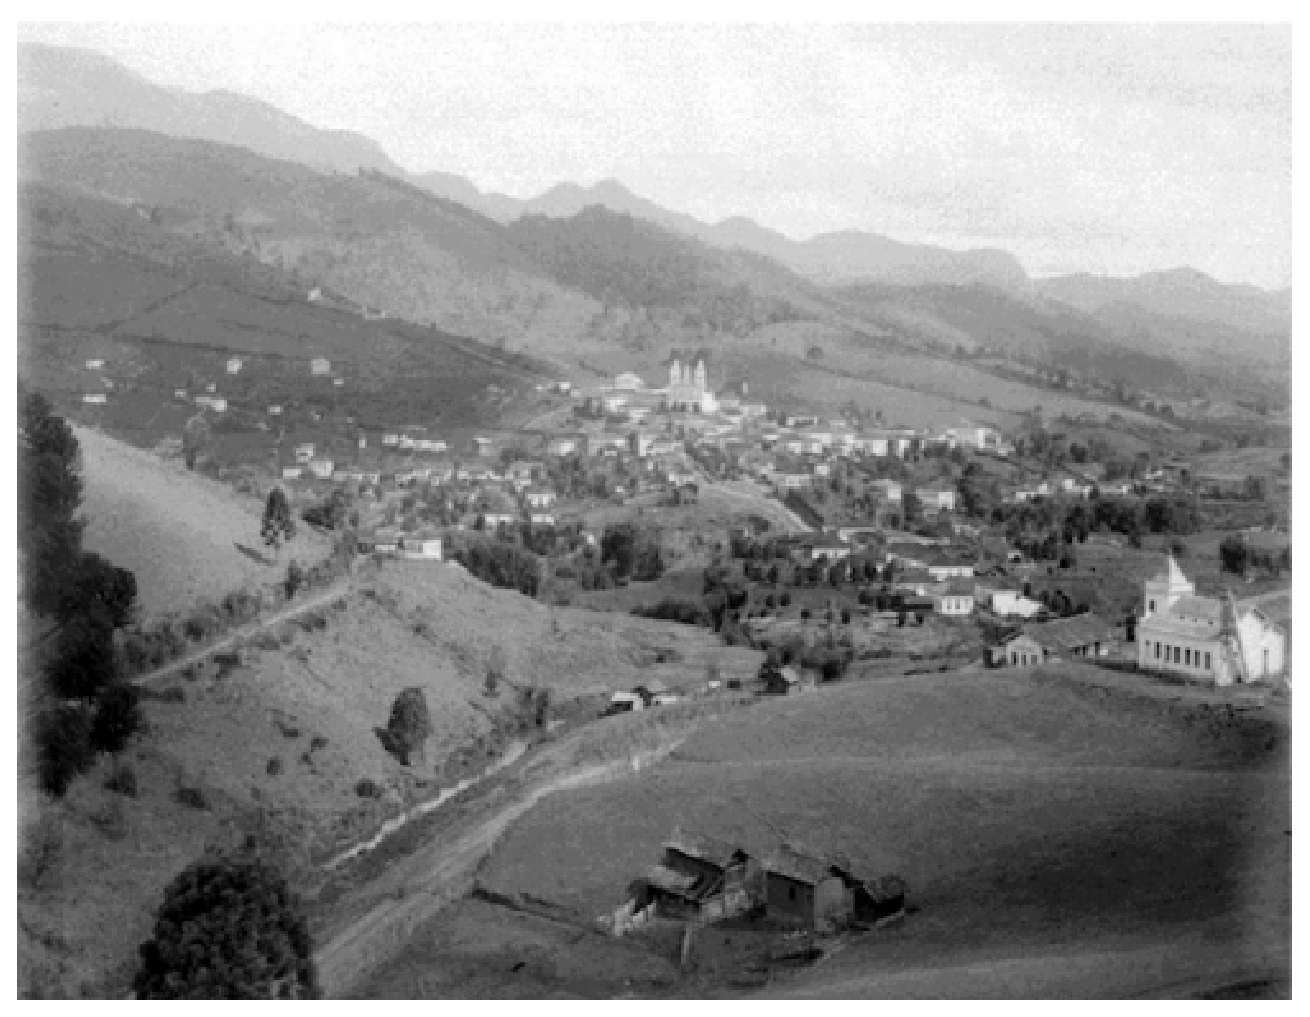
\includegraphics[width=0.5\textwidth]{figs/p1912.eps}
\end{figure}




% =============================================================================
% Smart Contracts
% =============================================================================
\section{Context}
\label{section:context}
%


% =============================================================================
% POAP.xyz
% =============================================================================
\section{Developer tools}
\label{section:Eth721}
%
We consider that since astropy is the leading open developer toolkit for astronomical research reflected in the astropy  user and dev comits see \cite{ 2020ASPC..522..491T}, that it be used at t0 launchdate but details could even be revised later by governance.  The Etherium blockchain contains a type of smart contracts called NFT or non-fungable token.  This type of token is non-interchangable can be unique to preserve the notion of digital scarcity, and can be verified without any centralized organization required to authenticate it. These smart contracts can be used issue incentive rewards to nodes. A protocol build around 721 protocal includes POAP.xyz, ref(github address). This proof of attendance protcol can be used to validad the attendance of astronomical events, including virtual ones. The tokens can be exchanged for goods and services and soldon for fiat money.  


Data feeds will be entered into Oracles that will automatically via smart contracts provide incentive rewards to the node and user wallets.
%
POAP type proof of attendence protocol for meetings. To rewards students for attending and presenting their results in meetings.
%
\subsection{Hash Function Account}
We propose for any developer of Astropy core plus afiliated package models including co-authors are onboarded and in our model we apply the afilated package astropy Package astrobtc, recognizing the fact that Bitcoin has been the major asset class for the last 12 years that included several global crisis. 
%

Astropy proving to revolutionize astronomical data-reduction collaboration and is channelled through the open development of astronomy project Astropy. It involves IVOA's 20 member institution was originally much smaller and conceived by its founding members to be a large fraternal virtual observatory working seamlessly in perfect collaboration with no imposed boundaries other than those of the ethical nature. Today it consists of mostly national VO members as well as three very important international members that include: the European Space Agency, the European VO and the UK VO. The national members are: Argentina, Armenia, Australia, Brazil, Canada, China, \textit{Europe}, France, Germany, Hungary, India, Italy, Japan, Korea, Russia, Spain, Ukraine, the United Kingdom and the United States. This `paper' proposes to open the discussion on the adoption of Block-chain technology for IVOA for the open development of astronomy. It is written in the context of long term flaws experienced in the current development model paradigm that results in less than efficient research inventive mechanism and cyclic funding crisis as well as possibly serendipitous COVID-19 type pandemic that may become more frequent.
%
Aside from some issues as illustrated below that would pausibly affects any 'closed' development model for astronomy, or one determined by powerful central actors, one based on open Blockchain technology should, on the other hand preferable gravitate to real open development via carefully thought-out and implemented incentive mechanisms to foster collaboration in a more efficient way and lay the path to unprecedented scientific discovery and innovation. It is in this context that I invite the reader to contemplate on the opening discussion of IVOA in the field of tokenomics. 
%
Our analysis focuses on the US public university research system, some limited experience on the IVOA system and the Argentine, Australian astronomical research system. 
   
   Strong motivation for this discussion is based on the facts that:
   
\begin{itemize}
       \item A dwindling half-life for the Astronomy and astrophysics PhD majors in US, Australian \& British (etc,) public university system meaning astronomy and astrophysics is loosing a main investment, its researchers.  
       
       \item Shortfalls caused by ciclic funding crisis that affect education institutions, scientific research facilities observed as acute funding restrictions, cutbacks and "government shutdowns" and/or inflation in national currencies, is the elephant in the room that must be addressed.
\end{itemize}
       
       
This paper explores the use of "Blockchain Technology" for more efficient and sustainable growth in Astronomy collaboration via real open development

A
% =============================================================================
% SECTION CONCLUSIONS
% =============================================================================
\section{Conclusions and Future Work}
\label{sec:5}
%
In this study, we set ourself a task to discuss systemic issues that have hampered Open Development for Astronomy and propose an affiliated package to astropy AstroOD to build on the DEFI stack including the creation of wallets. This new package is required to be developed by the community and must be compatible with up-coming Python versions and be fully documented in a public repository. 
%
Future development will focus on the following three areas: incorporating
new features, improving documentation, and 
possible integration with tools for interactively analyzing features of development.

IAU and IVOA Astronomer data-base to validate loose KYC, coordinating contact with institutions. 

% =============================================================================
% SECTION Acknowledgments
% =============================================================================
\section{Acknowledgments}
SG acknowledges the New Virtual Observatory of Argentina (NOVA) and his selection as representative of Argentina on the IVOA-exec committee.

% =============================================================================
% SECTION BIBLIO
% =============================================================================
%
%\section*{References}
%\label{biblio}
\bibliographystyle{model2-names-astronomy}
\bibliography{ivoatoken}


\end{document}

\endinput